\documentclass[12pt,a4paper,portrait]{article}
%\setcounter{secnumdepth}{0}
\usepackage{gensymb}
\usepackage{pdflscape}
\usepackage{amsmath}
\usepackage{amssymb}
\usepackage{enumitem}
\usepackage{graphicx}
\usepackage{subcaption}
\usepackage{multirow}
\usepackage{sansmath}
\usepackage{pst-eucl}
\usepackage{multicol}
\usepackage{csquotes}
% Coding
\usepackage{listings}
\setlength{\parindent}{0pt}
\usepackage[obeyspaces]{url}
% Better inline directory listings
\usepackage{xcolor}
\definecolor{light-gray}{gray}{0.95}
\newcommand{\code}[1]{\colorbox{light-gray}{\texttt{#1}}}
\usepackage{adjustbox}
\usepackage[UKenglish]{isodate}
\usepackage[UKenglish]{babel}
\usepackage{float}
\usepackage[T1]{fontenc}
\usepackage{setspace}
\usepackage{sectsty}
\usepackage{longtable}
\newenvironment{tightcenter}{%
	\setlength\topsep{0pt}
	\setlength\parskip{0pt}
	\begin{center}
	}{%
	\end{center}
}
\captionsetup{width=\textwidth}
\usepackage{mbenotes} % to print table notes!
\usepackage{alphalph} % For extended counters!
% usage: \tabnotemark[3]\cmsp\tabnotemark[4]
\usepackage[colorlinks=true,linkcolor=blue,urlcolor=black,bookmarksopen=true]{hyperref}
\sectionfont{%			            % Change font of \section command
	\usefont{OT1}{phv}{b}{n}%		% bch-b-n: CharterBT-Bold font
	\sectionrule{0pt}{0pt}{-5pt}{3pt}}
\subsectionfont{
	\usefont{OT1}{phv}{b}{n}}
\newcommand{\MyName}[1]{ % Name
	\usefont{OT1}{phv}{b}{n} \begin{center}of {\LARGE  #1}\end{center}
	\par \normalsize \normalfont}
\makeatletter
\newcommand\FirstWord[1]{\@firstword#1 \@nil}%
\newcommand\@firstword{}%
\newcommand\@removecomma{}%
\def\@firstword#1 #2\@nil{\@removecomma#1,\@nil}%
\def\@removecomma#1,#2\@nil{#1}
\makeatother

\newcommand{\MyTitle}[1]{ % Name
	\Huge \usefont{OT1}{phv}{b}{n} \begin{center}#1\end{center}
	\par \normalsize \normalfont}
\newcommand{\NewPart}[1]{\section*{\uppercase{#1}}}
\newcommand{\NewSubPart}[1]{\subsection*{\hspace{0.2cm}#1}}
\newcommand{\lag}{\mathcal{L}}
\renewcommand{\baselinestretch}{1.05}
\usepackage[margin=0.2cm]{geometry}
\date{}
\title{Pendulum on a cart on an inclined plane}
\author{Brenton Horne}

\begin{document}
	\maketitle
	\begin{figure}[H]
		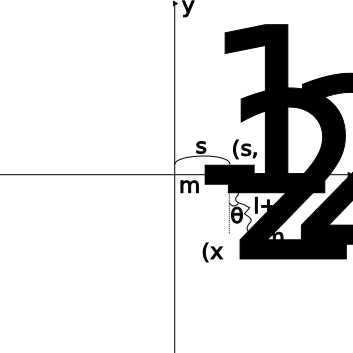
\includegraphics[width=500px]{Elastic pendulum on a cart.png}
		\caption{Diagram of problem.}\label{fig1}
	\end{figure}
	
	Here we have a cart whose centre of mass is at $(s, 0)$ and a pendulum attached to its horizontal centre bottom. To simplify calculations, we will assume the height of the cart is 0, but adding a constant height to the cart will not change the equations of motion.
	
	\tableofcontents
	\section{Coordinates, velocity and kinetic energy}
	Hence the kinetic energy for the cart is $\dfrac{m_1}{2}\dot{s}^2$. Next, we will calculate the coordinates, velocity and kinetic energy of the pendulum
	
	\begin{align*}
		x_2 &= s + (l+z)\sin{\theta} \\
		\dot{x}_2 &= \dot{s} + \dot{z}\sin{\theta} + (l+z)\dot{\theta}\cos{\theta}\\
		y_2 &= -(l+z)\cos{\theta} \\
		\dot{y}_2 &= -\dot{z}\cos{\theta} + (l+z)\dot{\theta}\sin{\theta} \\
		v_2^2 &= \dot{x}_2^2 + \dot{y}_2^2 \\
		&= (\dot{s} + \dot{z}\sin{\theta} + (l+z)\dot{\theta}\cos{\theta})^2 + (-\dot{z}\cos{\theta} + (l+z)\dot{\theta}\sin{\theta})^2 \\
		&= \dot{s}^2 + \dot{z}^2 \sin^2{\theta} + (l+z)^2\dot{\theta}^2\cos^2{\theta} + 2\dot{s}\dot{z}\sin{\theta} + 2\dot{s}\dot{\theta}(l+z)\cos{\theta} + 2\dot{z}\dot{\theta}(l+z)\sin{\theta}\cos{\theta} + \dot{z}^2\cos^2{\theta} \\
		&+ (l+z)^2\dot{\theta}^2\sin^2{\theta} - 2\dot{z}\dot{\theta}(l+z)\cos{\theta}\sin{\theta}\\
		&= \dot{s}^2 + \dot{z}^2 + (l+z)^2\dot{\theta}^2 + 2\dot{s}(\dot{z}\sin{\theta} + \dot{\theta}(l+z)\cos{\theta})\\
		T_p &= \dfrac{m_2}{2} \left(\dot{s}^2 + \dot{z}^2 + (l+z)^2\dot{\theta}^2 + 2\dot{s}(\dot{z}\sin{\theta} + \dot{\theta}(l+z)\cos{\theta})\right).
	\end{align*}
	
	Hence the total kinetic energy of the system is
	
	\begin{align*}
		T &= T_c + T_p \\
		&= \dfrac{m_1}{2}\dot{s}^2 + \dfrac{m_2}{2} \left(\dot{s}^2 + \dot{z}^2 + (l+z)^2\dot{\theta}^2 + 2\dot{s}(\dot{z}\sin{\theta} + \dot{\theta}(l+z)\cos{\theta})\right) \\
		&= \dfrac{m_1+m_2}{2} \dot{s}^2 + \dfrac{m_2}{2}\left(\dot{z}^2 + (l+z)^2\dot{\theta}^2 + 2\dot{s}(\dot{z}\sin{\theta} + \dot{\theta}(l+z)\cos{\theta})\right).
	\end{align*}
	
	\section{Potential energy}
	As for the potential energy, it comes in two forms --- gravitational and spring. 
	
	\begin{align*}
		V &= m_2 g y_2 + \dfrac{kz^2}{2}\\
		&= -m_2g(l+z)\cos{\theta} + \dfrac{kz^2}{2}.
	\end{align*}
	
	\section{Lagrangian}
	Hence the Lagrangian is
	
	\begin{align*}
		\lag &= T - V \\
		&= \dfrac{m_1+m_2}{2} \dot{s}^2 + \dfrac{m_2}{2}\left(\dot{z}^2 + (l+z)^2\dot{\theta}^2 + 2\dot{s}(\dot{z}\sin{\theta} + \dot{\theta}(l+z)\cos{\theta})+2g(l+z)\cos{\theta}\right) - \dfrac{kz^2}{2}.
	\end{align*}
	
	\section{Euler-Lagrange equations}
	The Euler-Lagrange equations for this system are
	
	\begin{align*}
		\dfrac{d}{dt}\dfrac{\partial \lag}{\partial \dot{q}_i} - \dfrac{\partial \lag}{\partial q_i} &= \sum_{j} \vec{F}_{D, j} \cdot \dfrac{\partial \vec{r}_{j}}{\partial q_i}
	\end{align*}
	
	where $j$ refers to the particles in the system. Or, defining
	
	\begin{align*}
		p_i &= \dfrac{\partial \lag}{\partial \dot{q}_i} & \dot{p}_i &= \dfrac{dp_i}{dt} \\
		F_i &= \dfrac{\partial \lag}{\partial q_i} & &= \dfrac{d}{dt}\dfrac{\partial \lag}{\partial \dot{q}_i}\\
		\hat{e}_{i,j} &= \dfrac{\partial \vec{r}_{j}}{\partial q_i} & Q_i &= \sum_{j} \vec{F}_{D, j} \cdot \hat{e}_{i,j}
	\end{align*}
	
	\subsection{$\theta$}
	\begin{align*}
		p_{\theta} &= \dfrac{\partial \lag}{\partial \dot{\theta}} \\
		&= m_2 \left[(l+z)^2 \dot{\theta} + \dot{s}(l+z)\cos{\theta}\right] \\
		\dot{p}_{\theta} &= m_2\left[2(l+z)\dot{z}\dot{\theta} + (l+z)^2\ddot{\theta} + \ddot{s}(l+z)\cos{\theta} + \dot{s}\dot{z}\cos{\theta} - \dot{s}(l+z)\dot{\theta}\sin{\theta}\right] \\
		&= m_2 \left[(l+z)^2 \ddot{\theta} + (l+z)\left(\dot{\theta}(2\dot{z} - \dot{s}\sin{\theta}) + \ddot{s}\cos{\theta}\right) + \dot{s}\dot{z}\cos{\theta}\right]\\
		F_{\theta} &= \dfrac{\partial \lag}{\partial \theta} \\
		&= \dfrac{\partial \lag}{\partial \theta} \\
		&= m_2(\dot{s}(\dot{z}\cos{\theta} - \dot{\theta}(l+z)\sin{\theta}) - g(l+z)\sin{\theta})\\
		&= m_2(\dot{s}\dot{z}\cos{\theta}-(l+z)\sin{\theta}(g+\dot{s}\dot{\theta})) \\
		Q_{\theta} &= \vec{F}_{D,cart} \cdot \hat{e}_{\theta,cart} + \vec{F}_{D,bob} \cdot \hat{e}_{\theta,bob} \\
		&= -(b_{cart}+c_{cart}|\dot{s}|)\begin{bmatrix}
			\dot{s}\\
			0
		\end{bmatrix} \cdot \vec{0}\\
		&-(b_{bob}+c_{bob}\sqrt{\dot{s}^2 + \dot{z}^2 + (l+z)^2\dot{\theta}^2 + 2\dot{s}(\dot{z}\sin{\theta} + \dot{\theta}(l+z)\cos{\theta})})\begin{bmatrix}
		\dot{s} + \dot{z}\sin{\theta} + (l+z)\dot{\theta}\cos{\theta} \\
		-\dot{z}\cos{\theta} + (l+z)\dot{\theta}\sin{\theta}
		\end{bmatrix} \cdot (l+z)\begin{bmatrix}
		\cos{\theta} \\
		\sin{\theta}
		\end{bmatrix} \\
		&= -(b_{bob}+c_{bob}\sqrt{\dot{s}^2 + \dot{z}^2 + (l+z)^2\dot{\theta}^2 + 2\dot{s}(\dot{z}\sin{\theta} + \dot{\theta}(l+z)\cos{\theta})})(l+z)\left(\dot{s}\cos{\theta} + \dot{z}\sin{\theta}\cos{\theta} + (l+z)\dot{\theta}\cos^2{\theta}\right.\\
		&\left.-\dot{z}\cos{\theta}\sin{\theta} + (l+z)\dot{\theta}\sin^2{\theta}\right) \\
		&= -(b_{bob}+c_{bob}\sqrt{\dot{s}^2 + \dot{z}^2 + (l+z)^2\dot{\theta}^2 + 2\dot{s}(\dot{z}\sin{\theta} + \dot{\theta}(l+z)\cos{\theta})})(l+z)\left(\dot{s}\cos{\theta}+(l+z)\dot{\theta}\right).
	\end{align*}
	
	Hence the Euler-Lagrange equation is
	
	\begin{align*}
		m_2 \left[(l+z)^2 \ddot{\theta} + (l+z)\left(\dot{\theta}(2\dot{z} - \dot{s}\sin{\theta}) + \ddot{s}\cos{\theta}\right) + \dot{s}\dot{z}\cos{\theta}\right] - m_2(\dot{s}\dot{z}\cos{\theta}-(l+z)\sin{\theta}(g+\dot{s}\dot{\theta})) &= Q_{\theta}\\
		(l+z)^2 \ddot{\theta} + (l+z)\left(\dot{\theta}(2\dot{z} - \dot{s}\sin{\theta}) + \ddot{s}\cos{\theta}\right) + \dot{s}\dot{z}\cos{\theta} - \dot{s}\dot{z}\cos{\theta}+(l+z)\sin{\theta}(g+\dot{s}\dot{\theta}) &= \dfrac{Q_{\theta}}{m_2} \\
		(l+z)^2 \ddot{\theta} + (l+z)(2\dot{z}\dot{\theta} + \ddot{s}\cos{\theta}+g\sin{\theta}) &= \dfrac{Q_{\theta}}{m_2}
	\end{align*}
	
	Hence
	
	\begin{align}
		\ddot{\theta} = -\dfrac{2\dot{z}\dot{\theta}+\ddot{s}\cos{\theta} + g\sin{\theta}}{l+z} + \dfrac{Q_{\theta}}{m_2(l+z)^2}.\label{d2theta1}
	\end{align}
	
	\subsection{$s$}
	\begin{align*}
		p_s &= \dfrac{\partial \lag}{\partial \dot{s}} \\
		&= (m_1+m_2)\dot{s} + m_2(\dot{z}\sin{\theta} + \dot{\theta}(l+z)\cos{\theta}) \\
		\dot{p}_s &= (m_1+m_2)\ddot{s} + m_2(\ddot{z}\sin{\theta}+\dot{z}\dot{\theta}\cos{\theta}+\ddot{\theta}(l+z)\cos{\theta}-\dot{\theta}^2(l+z)\sin{\theta}+\dot{\theta}\dot{z}\cos{\theta}) \\
		&= (m_1+m_2)\ddot{s} + m_2(\sin{\theta}(\ddot{z}-\dot{\theta}^2(l+z))+\cos{\theta}(2\dot{z}\dot{\theta}+\ddot{\theta}(l+z)))\\
		F_{s} &= \dfrac{\partial \lag}{\partial s} \\
		&= 0 \\
		\vec{F}_{D,cart} &= -(b_{cart}+c_{cart}|\dot{s}|)\begin{bmatrix}
			\dot{s}\\
			0
		\end{bmatrix} \\
		\vec{F}_{D,bob} &= -(b_{bob}+c_{bob}\sqrt{\dot{s}^2 + \dot{z}^2 + (l+z)^2\dot{\theta}^2 + 2\dot{s}(\dot{z}\sin{\theta} + \dot{\theta}(l+z)\cos{\theta})})\begin{bmatrix}
			\dot{s} + \dot{z}\sin{\theta} + (l+z)\dot{\theta}\cos{\theta} \\
			-\dot{z}\cos{\theta} + (l+z)\dot{\theta}\sin{\theta}
		\end{bmatrix} \\
		\hat{e}_{s, cart} &= \dfrac{\partial \vec{r}_{cart}}{\partial s} \\
		&= \begin{bmatrix}
			1 \\
			0
		\end{bmatrix} \\
		\hat{e}_{z, cart} &= \vec{0} \\
		\hat{e}_{\theta, cart} &= \vec{0} \\
		\hat{e}_{s, bob} &= \dfrac{\partial \vec{r}_{bob}}{\partial s} \\
		&= \begin{bmatrix}
			1 \\
			0
		\end{bmatrix} \\
		\hat{e}_{z, bob} &= \dfrac{\partial \vec{r}_{bob}}{\partial z} \\
		&= \begin{bmatrix}
			\sin{\theta}\\
			-\cos{\theta}
		\end{bmatrix} \\
		\hat{e}_{\theta, bob} &= \dfrac{\partial \vec{r}_{bob}}{\partial \theta} \\
		&= (l+z)\begin{bmatrix}
			\cos{\theta} \\
			\sin{\theta}
		\end{bmatrix}\\
		Q_s &= -(b_{cart}+c_{cart}|\dot{s}|)\dot{s} \\
		& -(b_{bob}+c_{bob}\sqrt{\dot{s}^2 + \dot{z}^2 + (l+z)^2\dot{\theta}^2 + 2\dot{s}(\dot{z}\sin{\theta} + \dot{\theta}(l+z)\cos{\theta})})\begin{bmatrix}
			\dot{s} + \dot{z}\sin{\theta} + (l+z)\dot{\theta}\cos{\theta} \\
			-\dot{z}\cos{\theta} + (l+z)\dot{\theta}\sin{\theta}
		\end{bmatrix} \cdot \begin{bmatrix}
		1 \\
		0
		\end{bmatrix} \\
		&= -(b_{cart}+c_{cart}|\dot{s}|)\dot{s} -\left(b_{bob}+c_{bob}\sqrt{\dot{s}^2 + \dot{z}^2 + (l+z)^2\dot{\theta}^2 + 2\dot{s}(\dot{z}\sin{\theta} + \dot{\theta}(l+z)\cos{\theta})}\right)(\dot{s} + \dot{z}\sin{\theta} \\
		&+ (l+z)\dot{\theta}\cos{\theta}) \\
		\therefore \ddot{s} &= -\dfrac{m_2}{m_1+m_2}\left[\sin{\theta}(\ddot{z}-\dot{\theta}^2(l+z))+\cos{\theta}(2\dot{z}\dot{\theta}+\ddot{\theta}(l+z))\right] + \dfrac{Q_s}{m_1+m_2}.
	\end{align*}
	
	Substituting Equation \eqref{d2theta1} in yields
	
	\begin{align*}
		\ddot{s} &= -\dfrac{m_2}{m_1+m_2}\left[\sin{\theta}(\ddot{z}-\dot{\theta}^2(l+z))+\cos{\theta}\left(2\dot{z}\dot{\theta}+(l+z)\left[-\dfrac{2\dot{z}\dot{\theta}+\ddot{s}\cos{\theta} + g\sin{\theta}}{l+z} + \dfrac{Q_{\theta}}{m_2(l+z)^2}\right]\right)\right] + \dfrac{Q_s}{m_1+m_2}\\
		&= -\dfrac{m_2}{m_1+m_2}\left[\sin{\theta}(\ddot{z}-\dot{\theta}^2(l+z))+\cos{\theta}\left(2\dot{z}\dot{\theta}-(2\dot{z}\dot{\theta}+\ddot{s}\cos{\theta} + g\sin{\theta}) + \dfrac{Q_{\theta}}{m_2(l+z)}\right)\right] + \dfrac{Q_s}{m_1+m_2} \\
		&=-\dfrac{m_2}{m_1+m_2}\left[\sin{\theta}(\ddot{z}-\dot{\theta}^2(l+z))-\ddot{s}\cos^2{\theta} - g\sin{\theta}\cos{\theta} + \dfrac{Q_{\theta}\cos{\theta}}{m_2(l+z)}\right] + \dfrac{Q_s}{m_1+m_2}
	\end{align*}
	Bringing all $\ddot{s}$ terms to the left-hand side
	\begin{align*}
		\ddot{s}\left(1-\dfrac{m_2\cos^2{\theta}}{m_1+m_2}\right) &= -\dfrac{m_2}{m_1+m_2}\left[\sin{\theta}(\ddot{z}-\dot{\theta}^2(l+z)) - g\sin{\theta}\cos{\theta} + \dfrac{Q_{\theta}\cos{\theta}}{m_2(l+z)}\right] + \dfrac{Q_s}{m_1+m_2}
	\end{align*}
	
	\begin{align*}
		1-\dfrac{m_2\cos^2{\theta}}{m_1+m_2} &= \dfrac{m_1+m_2 - m_2\cos^2{\theta}}{m_1+m_2} \\
		&= \dfrac{m_1+m_2\sin^2{\theta}}{m_1+m_2}.
	\end{align*}
	
	Therefore
	
	\begin{align}
		\ddot{s} &= -\dfrac{m_2}{m_1+m_2\sin^2{\theta}}\left[\sin{\theta}(\ddot{z}-\dot{\theta}^2(l+z)) - g\sin{\theta}\cos{\theta} + \dfrac{Q_{\theta}\cos{\theta}}{m_2(l+z)}\right] + \dfrac{Q_s}{m_1+m_2\sin^2{\theta}} \nonumber\\
		&= \dfrac{1}{m_1+m_2\sin^2{\theta}}\left[Q_s - \dfrac{Q_{\theta}\cos{\theta}}{l+z} - m_2\left(\sin{\theta}(\ddot{z}-\dot{\theta}^2(l+z)) - g\sin{\theta}\cos{\theta}\right)\right] \label{d2s1}
	\end{align}
	
	\section{$z$}
	\begin{align*}
		p_z &= \dfrac{\partial \lag}{\partial \dot{z}} \\
		&= m_2(\dot{z} + \dot{s}\sin{\theta}) \\
		\dot{p}_z &= m_2 (\ddot{z} + \ddot{s}\sin{\theta} + \dot{s}\dot{\theta}\cos{\theta})
	\end{align*}
	
	Substituting in Equation \eqref{d2s1}
	
	\begin{align*}
		\dot{p}_z &= m_2 \left[\ddot{z} + \sin{\theta}\left(\dfrac{1}{m_1+m_2\sin^2{\theta}}\left[Q_s - \dfrac{Q_{\theta}\cos{\theta}}{l+z} - m_2\left(\sin{\theta}(\ddot{z}-\dot{\theta}^2(l+z)) - g\sin{\theta}\cos{\theta}\right)\right]\right) + \dot{s}\dot{\theta}\cos{\theta}\right]\\
		&= m_2 \left[\ddot{z}\left(1-\dfrac{m_2\sin^2{\theta}}{m_1+m_2\sin^2{\theta}}\right) + \dfrac{\sin{\theta}}{m_1+m_2\sin^2{\theta}}\left[Q_s - \dfrac{Q_{\theta}\cos{\theta}}{l+z} + m_2\sin{\theta}\left(\dot{\theta}^2(l+z) + g\cos{\theta}\right)\right] + \dot{s}\dot{\theta}\cos{\theta}\right] \\
		&=m_2 \left[\dfrac{m_1\ddot{z}}{m_1+m_2\sin^2{\theta}} + \dfrac{\sin{\theta}}{m_1+m_2\sin^2{\theta}}\left[Q_s - \dfrac{Q_{\theta}\cos{\theta}}{l+z} + m_2\sin{\theta}\left(\dot{\theta}^2(l+z) + g\cos{\theta}\right)\right] + \dot{s}\dot{\theta}\cos{\theta}\right].
	\end{align*}
	
	\begin{align*}
		F_{z} &= \dfrac{\partial \lag}{\partial z} \\
		&= m_2\left((l+z)\dot{\theta}^2 + \dot{s}\dot{\theta}\cos{\theta} + g\cos{\theta}-k'z\right).
	\end{align*}
	
	Where $k'=\dfrac{k}{m_2}$. 	Finally, we will calculate $Q_z$
	
	\begin{align*}
		Q_z &= \vec{F}_{D,cart} \cdot \dfrac{\partial \vec{r}_{cart}}{\partial z} + \vec{F}_{D, bob} \cdot \dfrac{\partial \vec{r}_{bob}}{\partial z} \\
		&= -(b_{cart}+c_{cart}|\dot{s}|)\begin{bmatrix}
			\dot{s}\\
			0
		\end{bmatrix} \cdot \vec{0} -(b_{bob}+c_{bob}\sqrt{\dot{s}^2 + \dot{z}^2 + (l+z)^2\dot{\theta}^2 + 2\dot{s}(\dot{z}\sin{\theta} + \dot{\theta}(l+z)\cos{\theta})})\\
		&\begin{bmatrix}
			\dot{s} + \dot{z}\sin{\theta} + (l+z)\dot{\theta}\cos{\theta} \\
			-\dot{z}\cos{\theta} + (l+z)\dot{\theta}\sin{\theta}
		\end{bmatrix} \cdot \begin{bmatrix}
			\sin{\theta}\\
			-\cos{\theta}
		\end{bmatrix}\\
		&= -(b_{bob}+c_{bob}\sqrt{\dot{s}^2 + \dot{z}^2 + (l+z)^2\dot{\theta}^2 + 2\dot{s}(\dot{z}\sin{\theta} + \dot{\theta}(l+z)\cos{\theta})})
		(\dot{s}\sin{\theta} + \dot{z}\sin^2{\theta} + (l+z)\dot{\theta}\cos{\theta}\sin{\theta}\\
		&+\dot{z}\cos^2{\theta}- (l+z)\dot{\theta}\sin{\theta}\cos{\theta})\\
		&= -(b_{bob}+c_{bob}\sqrt{\dot{s}^2 + \dot{z}^2 + (l+z)^2\dot{\theta}^2 + 2\dot{s}(\dot{z}\sin{\theta} + \dot{\theta}(l+z)\cos{\theta})})
		(\dot{s}\sin{\theta} + \dot{z}).
	\end{align*}
	
	Hence the Euler-Lagrange equation is
	
	\begin{align*}
		&m_2 \left[\dfrac{m_1\ddot{z}}{m_1+m_2\sin^2{\theta}} + \dfrac{\sin{\theta}}{m_1+m_2\sin^2{\theta}}\left[Q_s - \dfrac{Q_{\theta}\cos{\theta}}{l+z} + m_2\sin{\theta}\left(\dot{\theta}^2(l+z) + g\cos{\theta}\right)\right] + \dot{s}\dot{\theta}\cos{\theta}\right] \\
		&- m_2\left((l+z)\dot{\theta}^2 + \dot{s}\dot{\theta}\cos{\theta} + g\cos{\theta}-k'z\right)= Q_z \\
	\end{align*}
	
	$m_2\dot{s}\dot{\theta}\cos{\theta}$ will be cancelled out. 
	
	Hence
	
	\begin{align*}
		\dfrac{m_1\ddot{z}}{m_1+m_2\sin^2{\theta}} + \dfrac{\sin{\theta}}{m_1+m_2\sin^2{\theta}}\left[Q_s - \dfrac{Q_{\theta}\cos{\theta}}{l+z} + m_2\sin{\theta}\left(\dot{\theta}^2(l+z) + g\cos{\theta}\right)\right] -(l+z)\dot{\theta}^2 - g\cos{\theta}+k'z &= \dfrac{Q_z}{m_2}
	\end{align*}
	\begin{align}
		\dfrac{m_1\ddot{z}}{m_1+m_2\sin^2{\theta}} &= -\dfrac{\sin{\theta}}{m_1+m_2\sin^2{\theta}}\left[Q_s - \dfrac{Q_{\theta}\cos{\theta}}{l+z} + m_2\sin{\theta}\left(\dot{\theta}^2(l+z) + g\cos{\theta}\right)\right] +(l+z)\dot{\theta}^2 + g\cos{\theta}+k'z + \dfrac{Q_z}{m_2} \nonumber\\
		&= \left[(l+z)\dot{\theta}^2+g\cos{\theta}\right]\left(1-\dfrac{m_2\sin^2{\theta}}{m_1+m_2\sin^2{\theta}}\right) -\dfrac{\sin{\theta}}{m_1+m_2\sin^2{\theta}}\left[Q_s - \dfrac{Q_{\theta}\cos{\theta}}{l+z} \right]+k'z + \dfrac{Q_z}{m_2}\label{d2z1}
	\end{align}
	
	\begin{align*}
		1-\dfrac{m_2\sin^2{\theta}}{m_1+m_2\sin^2{\theta}} &= \dfrac{m_1+m_2\sin^2{\theta}-m_2\sin^2{\theta}}{m_1+m_2\sin^2{\theta}}\\
		&= \dfrac{m_1}{m_1+m_2\sin^2{\theta}}.
	\end{align*}
	
	Multiplying both sides of Equation \eqref{d2z1} by $\dfrac{m_1+m_2\sin^2{\theta}}{m_1}$
	
	\begin{align}
		\ddot{z} &= (l+z)\dot{\theta}^2+g\cos{\theta} - \dfrac{\sin{\theta}}{m_1}\left[Q_s - \dfrac{Q_{\theta}\cos{\theta}}{l+z} \right]+\dfrac{m_1+m_2\sin^2{\theta}}{m_1m_2}\left(kz + Q_z\right) \label{d2z2}
	\end{align}
	
	Substituting into Equation \eqref{d2s1}:
	
	\begin{align*}
		\ddot{s} &= \dfrac{1}{m_1+m_2\sin^2{\theta}}\left[Q_s - \dfrac{Q_{\theta}\cos{\theta}}{l+z} - m_2\left(\sin{\theta}\left((l+z)\dot{\theta}^2+g\cos{\theta} - \dfrac{\sin{\theta}}{m_1}\left[Q_s - \dfrac{Q_{\theta}\cos{\theta}}{l+z} \right]\right.\right.\right.\\
		&\left.\left.\left.+\dfrac{m_1+m_2\sin^2{\theta}}{m_1m_2}\left(kz + Q_z\right)-\dot{\theta}^2(l+z)\right) - g\sin{\theta}\cos{\theta}\right)\right]
	\end{align*}
	Cancelling out the $\dot{\theta}^2(l+z)$ and $g\sin{\theta}\cos{\theta}$ terms
	\begin{align}
		\ddot{s} &= \dfrac{1}{m_1+m_2\sin^2{\theta}}\left[Q_s - \dfrac{Q_{\theta}\cos{\theta}}{l+z} +  \dfrac{m_2\sin^2{\theta}}{m_1}\left[Q_s - \dfrac{Q_{\theta}\cos{\theta}}{l+z} \right]\right.\nonumber\\
		&\left.-\dfrac{(m_1+m_2\sin^2{\theta})\sin{\theta}}{m_1}\left(kz + Q_z\right)\right]\nonumber\\
		&= \dfrac{1}{m_1+m_2\sin^2{\theta}}\left[\left(Q_s - \dfrac{Q_{\theta}\cos{\theta}}{l+z}\right)\left[1+\dfrac{m_2\sin^2{\theta}}{m_1}\right]-\dfrac{(m_1+m_2\sin^2{\theta})\sin{\theta}}{m_1}\left(kz + Q_z\right)\right]\nonumber\\
		&=  \dfrac{1}{m_1+m_2\sin^2{\theta}}\left[\left(Q_s - \dfrac{Q_{\theta}\cos{\theta}}{l+z}\right)\left[\dfrac{m_1+m_2\sin^2{\theta}}{m_1}\right]-\dfrac{(m_1+m_2\sin^2{\theta})\sin{\theta}}{m_1}\left(kz + Q_z\right)\right] \nonumber\\
		&= \dfrac{1}{m_1}\left(Q_s - \dfrac{Q_{\theta}\cos{\theta}}{l+z}\right) -\dfrac{(kz+Q_z)\sin{\theta}}{m_1} \nonumber\\
		&= \dfrac{1}{m_1}\left(Q_s - \dfrac{Q_{\theta}\cos{\theta}}{l+z}-(kz+Q_z)\sin{\theta}\right) \label{d2s}
	\end{align}
	
	Hence, substituting Equation \eqref{d2s} into \eqref{d2theta1} yields
	
	\begin{align*}
		\ddot{\theta} &= -\dfrac{2\dot{z}\dot{\theta}+\dfrac{\cos{\theta}}{m_1}\left(Q_s -(kz+Q_z)\sin{\theta}\right) + g\sin{\theta}}{l+z} + \dfrac{Q_{\theta}}{(l+z)^2m_1m_2}(m_1+m_2\cos^2{\theta})
	\end{align*}
\end{document}
	